Our current benchmarking evaluates how different GASing implementations handle specific mathematical sequences, such as: Fibonacci numbers, Factorial values, Powers of 2, Prime numbers, Repdigits (numbers with repeated digits), and Alternating digit patterns.

While these tests reveal that certain GASing implementations show clear advantages for specific patterns (e.g., the optimized C implementation excels at repdigit sequences due to efficient carry pattern recognition), the broader significance lies in the future direction of this benchmarking.

The following diagrams show the performance of different GASing implementations on digit-wise arithmetic operations based on String manipulation.

\begin{figure}[H]
  \centering
  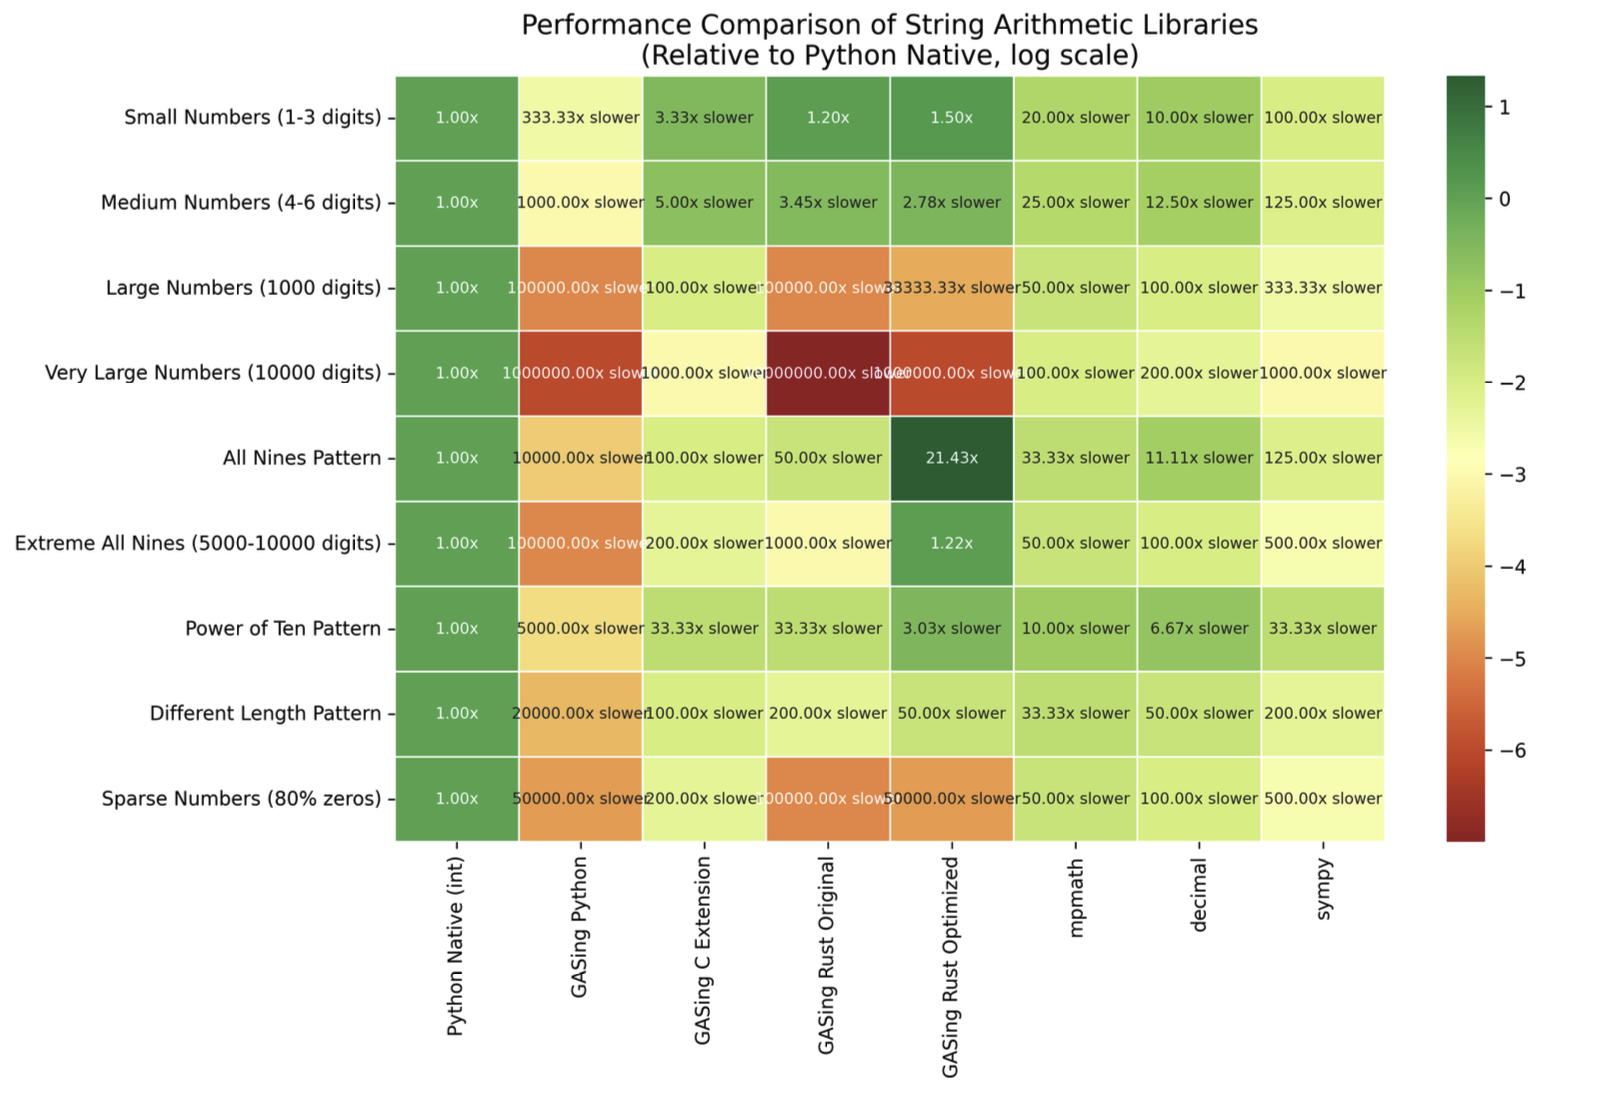
\includegraphics[width=\linewidth]{images/StringArithmetic.png}
  \caption{String Arithmetic}
  \label{fig:stringarithmetic}
\end{figure}



The following diagrams show the performance of different GASing implementations on the same set of algorithms applied to various number series for repeated applications of the same addition operations.

\begin{figure}[H]
  \centering
  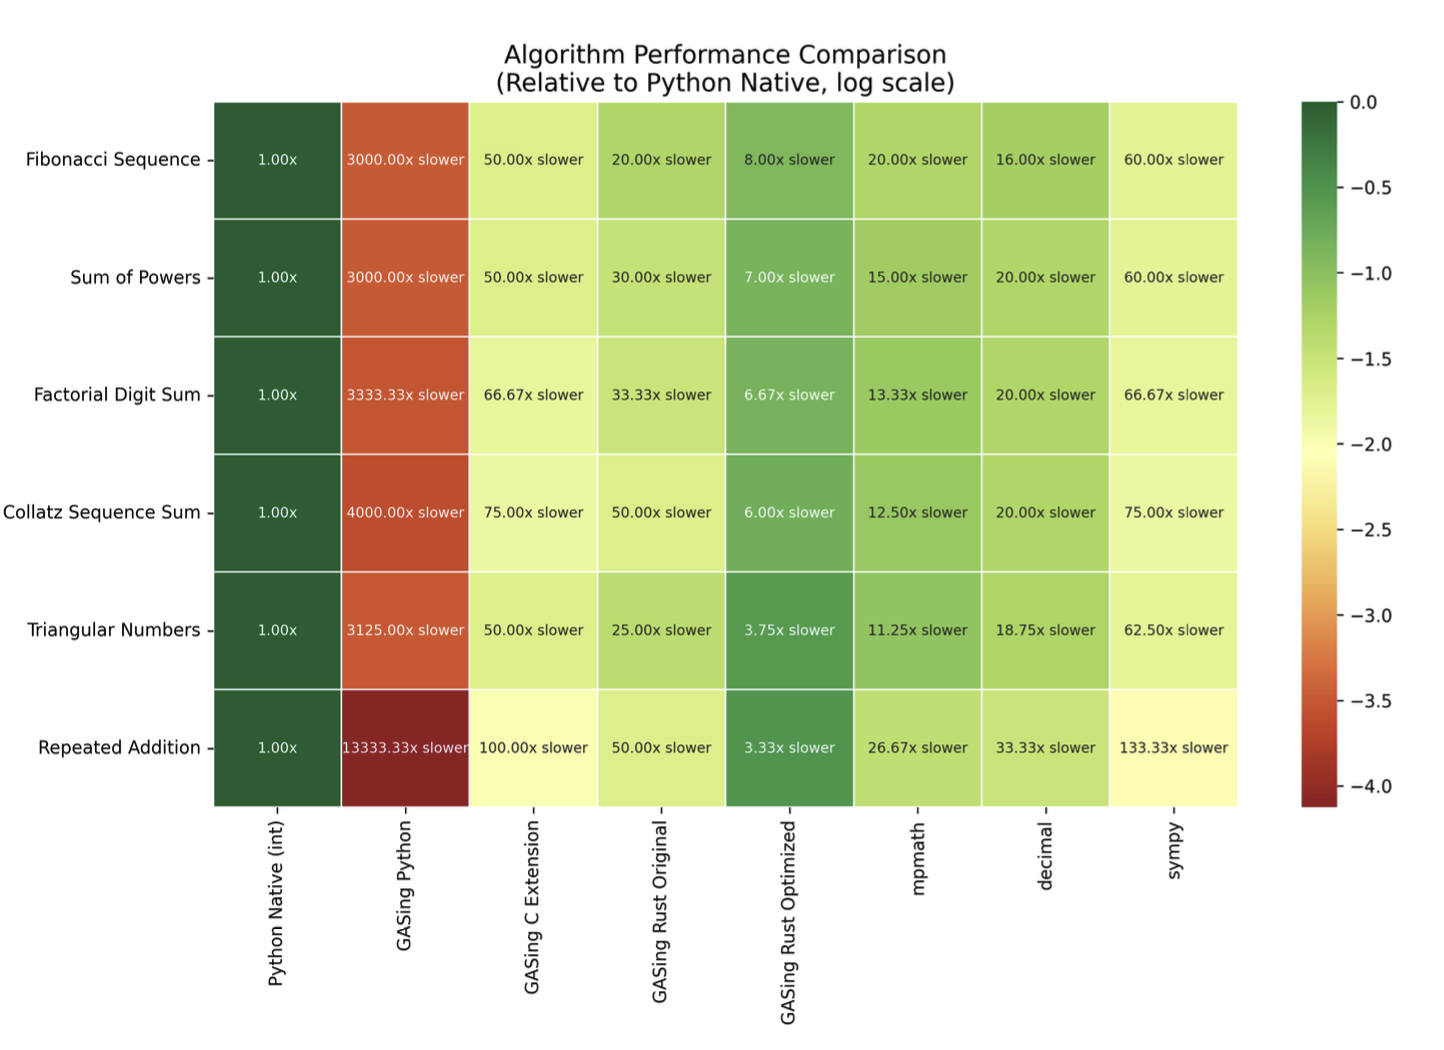
\includegraphics[width=\linewidth]{images/AlgorithmPerformanceComparison.png}
  \caption{Algorithmic Arithmetic}
  \label{fig:algorithmperformancecomparison}
\end{figure}



Looking ahead, these performance tests will be extended to arithmetic calculations that directly underpin large language model (LLM) inferencing. Since all inference operations in LLMs are ultimately arithmetic in nature—encompassing matrix multiplications, activations, and token transformations—any improvement in arithmetic efficiency translates directly to faster inference times and lower energy consumption at scale. This means that the resource savings demonstrated in these benchmarks could become highly visible and impactful in real-world AI deployments, especially as LLMs are deployed on increasingly resource-constrained or energy-sensitive platforms.

In summary, optimizing arithmetic operations through GASing principles has the potential to accelerate LLM inference, reduce operational costs, and make advanced AI systems more accessible and sustainable across a wide range of applications.
